\ylDisplay{Koer} % Ülesande nimi
{Tundmatu autor} % Autor
{lõppvoor} % Voor
{2012} % Aasta
{P 4} % Ülesande nr.
{2} % Raskustase
{
% Teema: Mehaanika

\ifStatement
Poiss on koos oma koeraga rannas. Joonisel kujutatud hetkel kutsub ta koera enda juurde, kuid koer soovib teel poisi juurde korraks ka veest läbi hüpata. Millise minimaalse ajaga jõuab ta sel juhul poisini? Koer jookseb kiirusega $v = 4,0$ m/s.
\begin{center}
	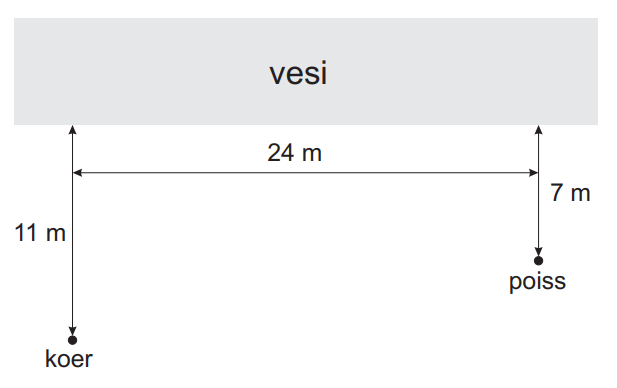
\includegraphics[width=0.5\linewidth]{2012-v3p-04-yl.PNG}
\end{center}
\fi

\ifHint
Lahenduse leidmiseks võiks punkti $P$ asemel kasutada tema peegeldust veepiiri suhtes $P'$ . Selliselt saab konstrueerida täisnurkse kolmnurga, mida lahendama hakata.
\fi

\ifSolution
\begin{center}
	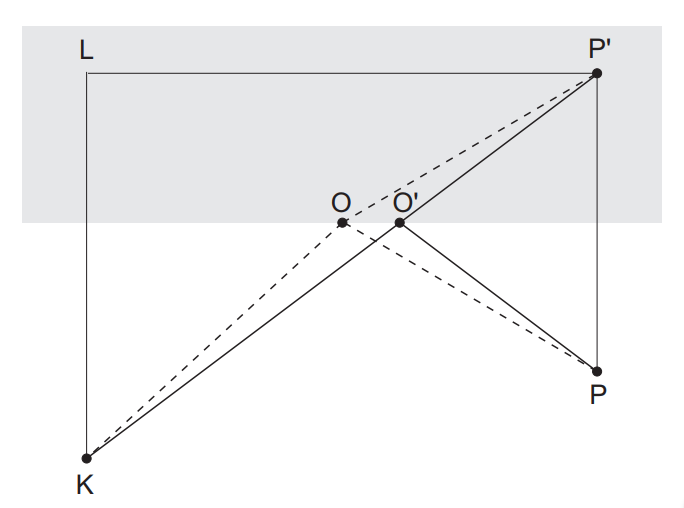
\includegraphics[width=0.5\linewidth]{2012-v3p-04-lah.PNG}
\end{center}
Oletame, et koer hüppab veest läbi punktis $O$ (vt joonist). Peegeldame poisi $P$ veepiiri suhtes, saame punkti $P'$. Paneme pähele, et $PO = PO'$, seega on teekond koera K juurest puntki $P'$ läbi punkti $O$ sama pikk, seega on teekond koera $K$ juurest punkti $P'$ läbi punkti $O$ sama pikk, kui teekond punkti P läbi punkti O. Lühim on see teekond juhul, kui tegemist on sirgega, mille korral koer hüppab veest läbi punktis $O'$.
\newline
Täisnurkses kolmnurgas $KLP'$ on $KL = 11 m + 7 m = 18$ $m$ ning $LP' = 24$ $m$. Niisiis $KP' = \sqrt{KL^2 + LP'^2} = 30$ m. Selle teekonna läbimiseks kulub aeg $KP' /v = 7.5$ s.
\fi
}